
\documentclass[11pt]{article}
\usepackage[margin=0.78in]{geometry}
\usepackage{booktabs}
\usepackage{graphicx}
\usepackage{float}
\usepackage{hyperref}
\hypersetup{colorlinks=true, linkcolor=blue, urlcolor=blue}
\title{Risk-Gated Transformer Selection Report}
\author{SPY American Call TP2 Project}
\date{\today}
\begin{document}
\maketitle

\section{Purpose}
This report evaluates a leakage-safe risk-gated selection layer on top of the corrected-history TP2-MV-ALiBi transformer. The transformer predictions are fixed. For each rolling fold, the policy and threshold are chosen using the validation year only. The test year is evaluated once.

\section{Selection Rule}
The candidate family includes probability floors, risk-aware objectives, and trade-count caps. A candidate is eligible only if validation P\&L is positive, validation trade count is at least 30, and its win-rate constraint is satisfied. The chosen candidate maximizes a validation-only robust score. No test-year P\&L is used to choose the policy or threshold.

\section{Aggregate Result}
\begin{table}[H]
\centering
\begin{tabular}{lr}
\toprule
Metric & Value \\
\midrule
Total selected trades & 86,921 \\
Total normalized P\&L & \$3,853,838 \\
Positive years & 4 / 6 \\
Combined Sharpe & 0.69 \\
Combined Sortino & 2.32 \\
Combined max drawdown & -\$3,681,550 \\
\bottomrule
\end{tabular}
\end{table}

\section{Yearly Results}
\begin{table}[H]
\centering
\small
\begin{tabular}{llrrrrrr}
\toprule
Year & Policy & Threshold & Trades & P\&L & Sharpe & Sortino & Max DD \\
\midrule
2021 & floor05_pnl & 0.17 & 16293 & \$3,681,383 & 2.09 & 10.08 & -\$847,508 \\
2022 & floor05_pnl & 0.05 & 6550 & -\$1,105,605 & -4.53 & -4.28 & -\$1,105,322 \\
2023 & floor05_pnl & 0.42 & 2106 & \$12,829 & 0.80 & 0.99 & -\$34,941 \\
2024 & floor05_pnl & 0.07 & 18560 & \$167,048 & 0.36 & 0.82 & -\$904,826 \\
2025 & floor05_pnl & 0.05 & 39160 & -\$1,128,548 & -0.74 & -1.95 & -\$3,537,886 \\
2026 & floor05_pnl & 0.05 & 4252 & \$2,226,731 & 3.21 & 91.66 & -\$128,175 \\
\bottomrule
\end{tabular}
\end{table}

\begin{figure}[H]
\centering
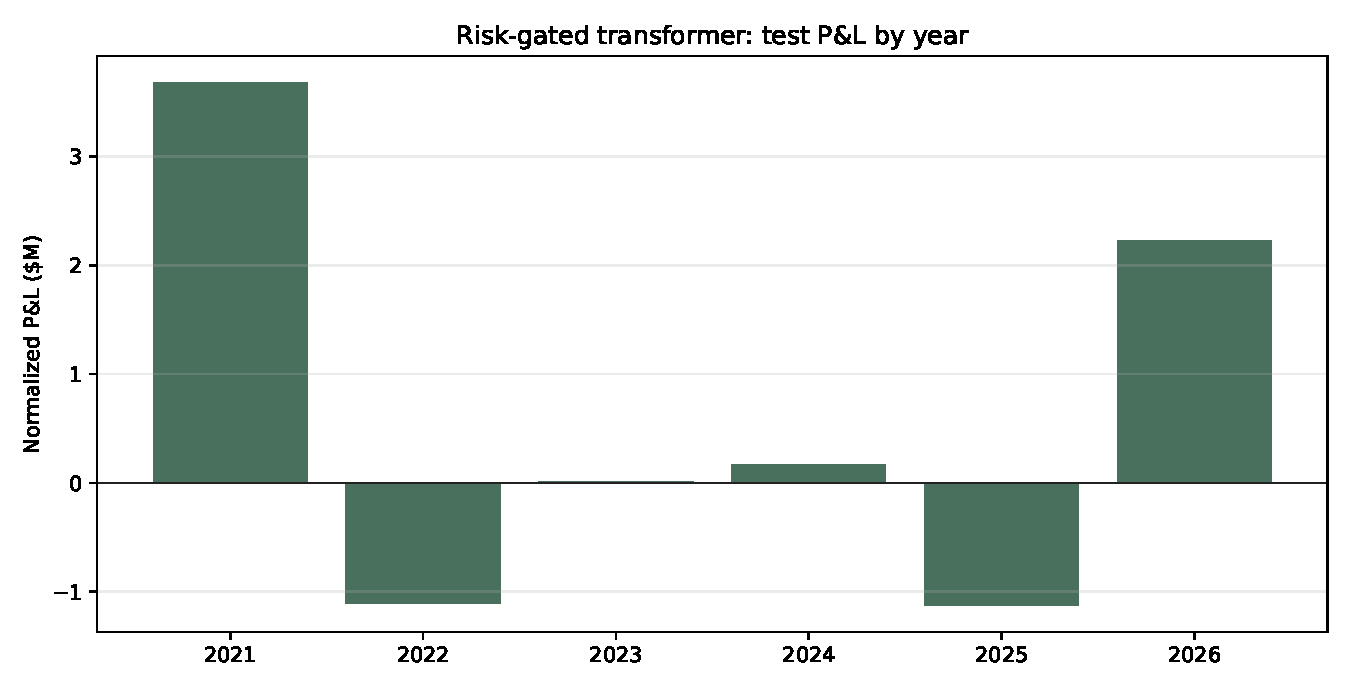
\includegraphics[width=0.88\linewidth]{figures/risk_gated_transformer_yearly_pnl.pdf}
\caption{Risk-gated transformer normalized P\&L by test year.}
\end{figure}

\begin{figure}[H]
\centering
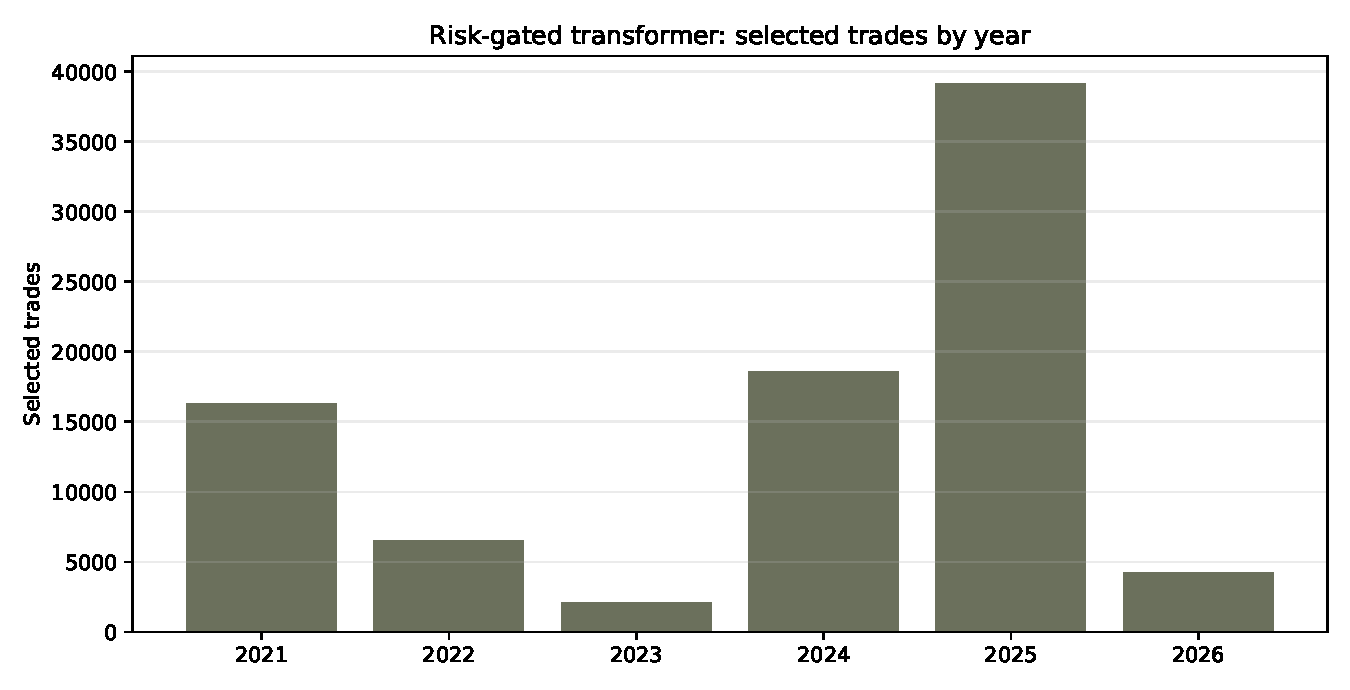
\includegraphics[width=0.88\linewidth]{figures/risk_gated_transformer_trade_counts.pdf}
\caption{Risk-gated transformer selected trades by test year.}
\end{figure}

\section{Interpretation}
This stage directly addresses the raw transformer's over-selection problem. If it improves worst-year behavior, the contribution is not merely the architecture; it is the combination of TP2-aware representation and validation-only risk-gated trade selection. If it remains weak, the next step should be feature/regime improvement rather than increasing transformer complexity.

\end{document}
